% Options for packages loaded elsewhere
\PassOptionsToPackage{unicode}{hyperref}
\PassOptionsToPackage{hyphens}{url}
\PassOptionsToPackage{dvipsnames,svgnames,x11names}{xcolor}
%
\documentclass[
  12pt,
]{scrreprt}
\usepackage{amsmath,amssymb}
\usepackage{lmodern}
\usepackage{iftex}
\ifPDFTeX
  \usepackage[T1]{fontenc}
  \usepackage[utf8]{inputenc}
  \usepackage{textcomp} % provide euro and other symbols
\else % if luatex or xetex
  \usepackage{unicode-math}
  \defaultfontfeatures{Scale=MatchLowercase}
  \defaultfontfeatures[\rmfamily]{Ligatures=TeX,Scale=1}
\fi
% Use upquote if available, for straight quotes in verbatim environments
\IfFileExists{upquote.sty}{\usepackage{upquote}}{}
\IfFileExists{microtype.sty}{% use microtype if available
  \usepackage[]{microtype}
  \UseMicrotypeSet[protrusion]{basicmath} % disable protrusion for tt fonts
}{}
\makeatletter
\@ifundefined{KOMAClassName}{% if non-KOMA class
  \IfFileExists{parskip.sty}{%
    \usepackage{parskip}
  }{% else
    \setlength{\parindent}{0pt}
    \setlength{\parskip}{6pt plus 2pt minus 1pt}}
}{% if KOMA class
  \KOMAoptions{parskip=half}}
\makeatother
\usepackage{xcolor}
\IfFileExists{xurl.sty}{\usepackage{xurl}}{} % add URL line breaks if available
\IfFileExists{bookmark.sty}{\usepackage{bookmark}}{\usepackage{hyperref}}
\hypersetup{
  pdftitle={ Digital Epigraphy in 2022},
  pdfauthor={Petra Heřmánková; Marietta Horster; Jonathan Prag},
  pdfkeywords={inscriptions, digital-epigraphy, FAIR data principles,
Linked Open Data, survey},
  colorlinks=true,
  linkcolor={Maroon},
  filecolor={Maroon},
  citecolor={cyan},
  urlcolor={blue},
  pdfcreator={LaTeX via pandoc}}
\urlstyle{same} % disable monospaced font for URLs
\usepackage[margin=1in]{geometry}
\usepackage{longtable,booktabs,array}
\usepackage{calc} % for calculating minipage widths
% Correct order of tables after \paragraph or \subparagraph
\usepackage{etoolbox}
\makeatletter
\patchcmd\longtable{\par}{\if@noskipsec\mbox{}\fi\par}{}{}
\makeatother
% Allow footnotes in longtable head/foot
\IfFileExists{footnotehyper.sty}{\usepackage{footnotehyper}}{\usepackage{footnote}}
\makesavenoteenv{longtable}
\usepackage{graphicx}
\makeatletter
\def\maxwidth{\ifdim\Gin@nat@width>\linewidth\linewidth\else\Gin@nat@width\fi}
\def\maxheight{\ifdim\Gin@nat@height>\textheight\textheight\else\Gin@nat@height\fi}
\makeatother
% Scale images if necessary, so that they will not overflow the page
% margins by default, and it is still possible to overwrite the defaults
% using explicit options in \includegraphics[width, height, ...]{}
\setkeys{Gin}{width=\maxwidth,height=\maxheight,keepaspectratio}
% Set default figure placement to htbp
\makeatletter
\def\fps@figure{htbp}
\makeatother
\setlength{\emergencystretch}{3em} % prevent overfull lines
\providecommand{\tightlist}{%
  \setlength{\itemsep}{0pt}\setlength{\parskip}{0pt}}
\setcounter{secnumdepth}{-\maxdimen} % remove section numbering
\newlength{\cslhangindent}
\setlength{\cslhangindent}{1.5em}
\newlength{\csllabelwidth}
\setlength{\csllabelwidth}{3em}
\newlength{\cslentryspacingunit} % times entry-spacing
\setlength{\cslentryspacingunit}{\parskip}
\newenvironment{CSLReferences}[2] % #1 hanging-ident, #2 entry spacing
 {% don't indent paragraphs
  \setlength{\parindent}{0pt}
  % turn on hanging indent if param 1 is 1
  \ifodd #1
  \let\oldpar\par
  \def\par{\hangindent=\cslhangindent\oldpar}
  \fi
  % set entry spacing
  \setlength{\parskip}{#2\cslentryspacingunit}
 }%
 {}
\usepackage{calc}
\newcommand{\CSLBlock}[1]{#1\hfill\break}
\newcommand{\CSLLeftMargin}[1]{\parbox[t]{\csllabelwidth}{#1}}
\newcommand{\CSLRightInline}[1]{\parbox[t]{\linewidth - \csllabelwidth}{#1}\break}
\newcommand{\CSLIndent}[1]{\hspace{\cslhangindent}#1}
\usepackage{booktabs}
\usepackage{longtable}
\usepackage{microtype}
\usepackage[bf,singlelinecheck=off]{caption}
\usepackage[scale=.8]{sourcecodepro}

\usepackage{framed,color}
\definecolor{shadecolor}{RGB}{248,248,248}


    \makeatletter
    %\let\@fnsymbol\@alph
    \let\@fnsymbol\@arabic
    \makeatother

%\renewcommand{\thefootnote}{\arabic{footnote}}
\ifLuaTeX
  \usepackage{selnolig}  % disable illegal ligatures
\fi

\title{
\includegraphics[width=3in,height=\textheight]{../assets/banner.png}\\
Digital Epigraphy in 2022\footnote{This work was supported by the Arts
  and Humanities Research Council (AHRC) {[}grant number
  AH/W010682/1{]}; and the Deutsche Forschungsgemeinschaft (DFG)
  {[}grant number 468455971{]}. The report is published via Zenodo,
  \url{https://doi.org/10.5281/zenodo.6610696}}}
\usepackage{etoolbox}
\makeatletter
\providecommand{\subtitle}[1]{% add subtitle to \maketitle
  \apptocmd{\@title}{\par {\large #1 \par}}{}{}
}
\makeatother
\subtitle{A Report from the Scoping Survey of the FAIR Epigraphy
Project}
\author{Petra Heřmánková\footnote{Johannes Gutenberg University in
  Mainz,
  \href{mailto:petra.hermankova@uni.mainz.de}{\nolinkurl{petra.hermankova@uni.mainz.de}},
  \url{https://orcid.org/0000-0002-6349-0540}} \and Marietta
Horster\footnote{Johannes Gutenberg University in Mainz, Corpus
  Inscriptionum Latinarum/BBAW,
  \href{mailto:horster@uni.mainz.de}{\nolinkurl{horster@uni.mainz.de}},
  \url{https://orcid.org/0000-0003-1434-224X}} \and Jonathan
Prag\footnote{University of Oxford,
  \href{mailto:jonathan.prag@merton.ox.ac.uk}{\nolinkurl{jonathan.prag@merton.ox.ac.uk}},
  \url{https://orcid.org/0000-0003-3819-8537}}}
\date{03 June, 2022}

\begin{document}
\maketitle
\begin{abstract}
This document maps the state of digital epigraphy in 2022, with a focus
on Open Science practices and accessibility of resources. The report is
based on anonymised responses received during the digital survey
circulating between February and April 2022, organised by the FAIR
Epigraphy Project. The responses cover a broad spectrum of projects from
Europe and the USA, ranging from well established projects with
relatively stable institutional support to short-term projects with more
narrow focus and limited access to IT support and funding. The results
of the survey will be used to inform the planning of the FAIR Epigraphy
project in the following three years. The report is fully reproducible
(written in R programming language) and along with the anonymised data
is accessible via its own GitHub repository
(\url{https://github.com/FAIR-epigraphy/scoping_survey_report}), and
published through Zenodo (\url{https://doi.org/10.5281/zenodo.6610696}).
\end{abstract}

{
\hypersetup{linkcolor=}
\setcounter{tocdepth}{2}
\tableofcontents
}
\hypertarget{introduction}{%
\chapter{Introduction}\label{introduction}}

The field of digital epigraphy has seen significant development in
recent years: not only are traditional epigraphic corpora increasingly
being digitised and made accessible via their websites for anyone to
browse and search but several resources are already born digital without
any printed edition, e.g.~\emph{Inscriptions of Greek Cyrenaica}
(\protect\hyperlink{ref-roueche_inscriptions_2020}{Roueche \emph{et
al.}, 2020}), \emph{Inscriptions of Roman Tripolitania}
(\protect\hyperlink{ref-roueche_inscriptions_2022}{Roueche, 2022}); for
more see (\protect\hyperlink{ref-bruun_epigraphy_2015}{Elliott, 2015}).
Most inscriptions contain references to places, people or events, or
contain data related to the place and time of their creation and provide
an ideal resource to study past communities as a whole. However, in
order to be able to harness their full potential and for example access
\emph{all} inscriptions from a place of interest or of a given type, we
need to link the existing datasets together. The concept of \emph{Linked
Open Data} (LOD) provides a means of connecting various digital datasets
while enriching the text with, e.g.~broader spatio-temporal context or
prosopographic data, leading to the creation of new connections between
individual inscriptions as well as archaeological sites or potential
re-evaluation of historical narratives
(\protect\hyperlink{ref-bagnall_pleiades_2006}{Bagnall \emph{et al.},
2006}; \protect\hyperlink{ref-geser_wp15_2016}{Geser, 2016};
\protect\hyperlink{ref-tupman_where_2021}{Tupman, 2021}). Although many
epigraphic datasets have been using LOD, especially to record the
spatial component by using services such as Pleiades or Trismegistos,
there is still a considerable gap in the LOD implementation across the
discipline and thus in the accessibility of the data.

An individual dataset that is not more widely accessible or
interoperable is of considerable value to groups sharing similar
interests (e.g.~geographic area, chronological period, linguistic
environment), but of much more limited value to the epigraphic
discipline as a whole. The value of LOD lies in being able to build on
the efforts and investment of numerous generations of epigraphers who
over many years have produced multiple high-quality editions in first
analogue and more recently also digital form. Whether there is one
master database connecting all the inscriptions together, or not, once
the data is \textbf{FAIR} (\emph{Findable}, \emph{Accessible},
\emph{Interoperable}, \emph{Reusable}
(\protect\hyperlink{ref-wilkinson_fair_2016}{Wilkinson \emph{et al.},
2016})) and linked to other LOD, new avenues of research open - either
to large scale, comparative studies such as
(\protect\hyperlink{ref-assael_restoring_2022}{Assael \emph{et al.},
2022}; \protect\hyperlink{ref-glomb_popularity_2022}{Glomb \emph{et
al.}, 2022};
\protect\hyperlink{ref-hermankova_inscriptions_2021}{Heřmánková \emph{et
al.}, 2021}) or projects working on the same material but with different
emphases (\protect\hyperlink{ref-mullen_manual_2021}{Mullen \& Bowman,
2021}; \protect\hyperlink{ref-willi_manual_2021}{Willi, 2021}). Once the
data is linked, there is no need to build one central repository, which
is often costly and unsustainable in the long run as documented by the
recent experience of the EAGLE Portal
(\protect\hyperlink{ref-orlandi_digital_2021}{Orlandi, 2021}), but
instead one can empower individual users and provide them with clear
guidelines and skills on how to work with LOD in epigraphy.

The \textbf{FAIR Epigraphy} Project
(\url{https://www.csad.ox.ac.uk/fair-epigraphy}) aims to fill in the gap
between the digitisation of inscriptions and the realisation of being
able to use their full potential as a digital resource. The FAIR
Epigraphy project has been established as a collaboration between
Johannes Gutenberg University in Mainz (Prof.~Marietta Horster) and the
University of Oxford (Prof.~Jonathan Prag), funded by the Arts and
Humanities Research Council (AHRC) and Deutsche Forschungemeinschaft
(DFG) and will run for 36 months, from 2022 to 2025. \textbf{FAIR
Epigraphy} aims to create an interactive platform for all epigraphic
projects, aligning their digital needs with the principles of FAIR
science. The overall desirability of \textbf{FAIR} - \emph{Findable},
\emph{Accessible}, \emph{Interoperable}, \emph{Reusable}
(\protect\hyperlink{ref-wilkinson_fair_2016}{Wilkinson \emph{et al.},
2016}) - data is fundamental for advancing research into the epigraphic,
linguistic, and material culture of the ancient world.

\begin{quote}
\emph{``The principles emphasise machine-actionability (i.e.~the
capacity of computational systems to find, access, interoperate, and
reuse data with none or minimal human intervention) because humans
increasingly rely on computational support to deal with data as a result
of the increase in volume, complexity, and creation speed of data.''}
(FAIR Principles website,
\url{https://www.go-fair.org/fair-principles/})
\end{quote}

With the increase in Linked Open Data and novel interface technologies
and standards, the FAIR Epigraphy Project will be able to create the
tools and the community needed to transform epigraphic research in the
digital age. However, FAIR Epigraphy does not wish to replicate any
current efforts, but rather to align existing initiatives and bring them
together to create a hub of high-quality tools and FAIR compliant
standards and resources for the modern epigraphic discipline. Our
internationally collaborative approach will enable and support
innovative research across epigraphic data and the wider linked web of
data (especially archaeological data), such that all epigraphic data is
increasingly FAIR for both the research community and the wider public.
To this end, we aim to:

\begin{enumerate}
\def\labelenumi{\arabic{enumi}.}
\tightlist
\item
  consolidate community-wide standards (vocabularies and ontology);
\item
  host and make fully accessible the resulting linked open data
  published by individual projects (RDF/XML data publication);
\item
  develop the tools for community implementation of those standards
  (vocabulary and ontology hosting and publication);
\item
  provide support to members of the community in implementing the
  standards within existing and new projects.
\end{enumerate}

In order to map the existing field of digital epigraphy including
current practices and standards, as well as to clarify the (digital)
needs of the discipline, we circulated two scoping surveys between
February and April 2022
(\href{https://github.com/FAIR-epigraphy/scoping_survey_report/data/01_Survey_partners_questions.pdf}{\textbf{FAIR
Epigraphy: Scoping survey for partners and collaborators}} and
\href{https://github.com/FAIR-epigraphy/scoping_survey_report/data/02_Survey_projects_questions.pdf}{\textbf{Digital
epigraphy in 2022: scoping survey}} for all digital epigraphy projects).
The results of the surveys presented in the current report will be used
to plan the activities and efficiently allocate the resources of the
FAIR Epigraphy Project in the following three years. The report contains
only the answers where participants gave consent to publish the
anonymised responses. In cases where the consent was not given, the data
is used to inform the FAIR Epigraphy decision but is excluded from the
report.

The survey answers are anonymised so that individual projects cannot be
identified on the basis of their replies and the data is stored as a TSV
(tab-separated value) file within the project's GitHub repository
(\url{https://github.com/FAIR-epigraphy/scoping_survey_report/}) as a
supplement to the text of this report and can be accessed under the
CC-BY-SA 4.0 International License. The report is produced in two
formats: a traditional PDF (available at
\url{https://github.com/FAIR-epigraphy/scoping_survey_report/blob/main/scripts/01_FAIR_epi_report.pdf})
and an interactive HTML page where the reader can browse through the
responses (available at
\url{https://fair-epigraphy.github.io/scoping_survey_report/scripts/01_FAIR_epi_report.html}).
\emph{If you are viewing this report in the HTML format, to browse the
data click on the arrow in the top right corner of the data tables in
each section (where the arrow is available).}

\textbf{Disclaimer}: The views and opinions expressed within the survey
(presented in tables) do not necessarily reflect the views or positions
of the FAIR Epigraphy Project itself.

\hypertarget{fair-epigraphy-partner-projects}{%
\chapter{FAIR Epigraphy partner
projects}\label{fair-epigraphy-partner-projects}}

\footnotesize

\normalsize

This section summarises the results of the online survey
\href{https://github.com/FAIR-epigraphy/scoping_survey_report/data/01_Survey_partners_questions.pdf}{\emph{FAIR
Epigraphy: Scoping survey for partners and collaborators}} aimed at
those established digital projects which are already official partners
and collaborators of the FAIR Epigraphy Project. We sent the survey to
14 partner projects. We received 13 responses to the survey, a response
rate of 93\% with some participants responding on behalf of two projects
combined into one response (and thus skewing the response rate). 100\%
of participating partner projects gave consent to publish their
anonymised responses as part of this report.

The partner projects represent successful projects with the average
duration of a project being 6 years. The shortest participating project
reported their duration as 3 years and the longest as 207
years.\footnote{Obviously not digital for the whole of that period.}

\hypertarget{language-coverage}{%
\section{Language coverage}\label{language-coverage}}

\textbf{Question:} \emph{What is the predominant language of epigraphic
data in your project (for mixed collections or collections where other
languages are predominant provide details in Other)}\footnote{If you are
  viewing this report in the HTML format, you can click on the arrow in
  the top right corner of the table to see more data (where available).
  This functionality is not available in the PDF format.}

\footnotesize

\begin{longtable}[]{@{}
  >{\raggedright\arraybackslash}p{(\columnwidth - 4\tabcolsep) * \real{0.8902}}
  >{\raggedleft\arraybackslash}p{(\columnwidth - 4\tabcolsep) * \real{0.0366}}
  >{\raggedleft\arraybackslash}p{(\columnwidth - 4\tabcolsep) * \real{0.0732}}@{}}
\toprule
\begin{minipage}[b]{\linewidth}\raggedright
language
\end{minipage} & \begin{minipage}[b]{\linewidth}\raggedleft
n
\end{minipage} & \begin{minipage}[b]{\linewidth}\raggedleft
ratio
\end{minipage} \\
\midrule
\endhead
Latin & 9 & 30 \\
Greek & 7 & 23 \\
Hebrew & 2 & 7 \\
Other & 2 & 7 \\
Ancient Celtic & 1 & 3 \\
Elymian & 1 & 3 \\
Etruscan & 1 & 3 \\
Gaulish & 1 & 3 \\
Oscan & 1 & 3 \\
other epichoric languages from the west provinces of Rome (excl. Africa)
& 1 & 3 \\
Phoenician-Punic & 1 & 3 \\
Punic & 1 & 3 \\
Raetic & 1 & 3 \\
Sikel & 1 & 3 \\
\bottomrule
\end{longtable}

\normalsize

\footnotesize

\normalsize

\textbf{Commentary:} The language coverage of the participating projects
consists predominantly of Latin and Greek either alone or in combination
(representing 53\% of the answers). 8 participating projects record
inscriptions in one language only, while 5 contain inscriptions in two
or more languages (7 being the maximum number of listed languages in one
project.)

The \texttt{Other} (i.e.~other than Greek and Latin) category
encompassed a substantial part of the surveyed projects (47\%),
documenting the need to expand beyond the traditional Latin and Greek
focus of the classical epigraphic discipline. The languages listed as
\texttt{Other} consisted of \emph{Other, Ancient Celtic, Elymian,
Etruscan, Gaulish, Oscan, other epichoric languages from the west
provinces of Rome (excl. Africa), Phoenician-Punic, Punic, Raetic,
Sikel}. It is, however, worth noting that the majority of participating
projects record languages from the wider Mediterranean/European
linguistic space.

\textbf{Unique combinations of languages as retrieved from the survey:}

\footnotesize

\begin{longtable}[]{@{}
  >{\raggedright\arraybackslash}p{(\columnwidth - 0\tabcolsep) * \real{1.0000}}@{}}
\toprule
\begin{minipage}[b]{\linewidth}\raggedright
unique(partners\$Language\_clean)
\end{minipage} \\
\midrule
\endhead
Greek; Latin \\
Latin \\
Gaulish \\
Latin; Greek; Punic; Etruscan; Hebrew; Raetic; Other \\
Latin; Greek; other epichoric languages from the west provinces of Rome
(excl. Africa) \\
Greek \\
Ancient Celtic \\
Latin; Greek; Other \\
Greek; Latin; Phoenician-Punic; Oscan; Sikel; Elymian; Hebrew \\
\bottomrule
\end{longtable}

\normalsize

\begin{center}\rule{0.5\linewidth}{0.5pt}\end{center}

\hypertarget{it-infrastructure}{%
\section{IT infrastructure}\label{it-infrastructure}}

\textbf{Question}: \emph{Does the project have a website?}

\footnotesize

\begin{longtable}[]{@{}lr@{}}
\toprule
Website & n \\
\midrule
\endhead
Yes & 13 \\
\bottomrule
\end{longtable}

\normalsize

\textbf{Commentary}: All of the participating projects currently
maintain an online presence (as of February-April 2022).

\begin{center}\rule{0.5\linewidth}{0.5pt}\end{center}

\textbf{Question}: \emph{Does your project have an IT specialist(s)?}

\footnotesize

\begin{longtable}[]{@{}
  >{\raggedright\arraybackslash}p{(\columnwidth - 4\tabcolsep) * \real{0.9492}}
  >{\raggedleft\arraybackslash}p{(\columnwidth - 4\tabcolsep) * \real{0.0169}}
  >{\raggedleft\arraybackslash}p{(\columnwidth - 4\tabcolsep) * \real{0.0339}}@{}}
\toprule
\begin{minipage}[b]{\linewidth}\raggedright
IT\_spec
\end{minipage} & \begin{minipage}[b]{\linewidth}\raggedleft
n
\end{minipage} & \begin{minipage}[b]{\linewidth}\raggedleft
ratio
\end{minipage} \\
\midrule
\endhead
Yes, equivalent of part-time (\textless1.0 FTE) position & 7 & 54 \\
No & 3 & 23 \\
We paid some specialists, but currently we have no budget for them (and
this is a problem, even for the sustainability and ordinary maintainance
of our digital assets) & 1 & 8 \\
Yes, equivalent of full-time (1.0 FTE) position & 1 & 8 \\
Yes, equivalent of more than full-time (\textgreater1.0 FTE) position &
1 & 8 \\
\bottomrule
\end{longtable}

\normalsize

\textbf{Commentary}: The majority of the digital partner projects have
an IT specialist, yet only 2 projects have an equivalent of 1.0 FTE or
more at their disposal. 54 \% of projects have access to part-time IT
support for their projects, which in some instances may be only a few
hours per week per project. 4 projects reported no availability of IT
support, even on a part-time basis (representing 31\% of participating
partner projects).

\begin{center}\rule{0.5\linewidth}{0.5pt}\end{center}

\textbf{Question}: \emph{Does your project store epigraphic data in the
following formats\ldots?}

\footnotesize

\begin{longtable}[]{@{}lrr@{}}
\toprule
format & n & no\_format \\
\midrule
\endhead
Epidoc XML & 4 & 1 \\
Epidoc XML, CSV, SQL or similar & 1 & 3 \\
Epidoc XML, in print & 1 & 2 \\
Epidoc XML, JSON, CSV & 1 & 3 \\
Epidoc XML, JSON, RDF & 1 & 3 \\
Epidoc XML, SQL or similar & 1 & 2 \\
None - we use analog systems (printed) & 1 & 1 \\
RDF, SQL or similar & 1 & 2 \\
SQL or similar & 1 & 1 \\
We aim to switch to Epidoc XML storable data & 1 & 1 \\
\bottomrule
\end{longtable}

\normalsize

\footnotesize

\normalsize

\textbf{Commentary}: The majority of projects use \texttt{Epidoc\ XML}
as their main output data format (77\% of participating projects),
either in combination with other formats or as the sole data format.
Other data formats are represented less frequently: JSON (15\%), RDF
(15\%), SQL (31\%) and CSV (15\%). 31\% of projects use only one type of
data format, while 46\% use two or more data format types within their
project.

\hypertarget{data-sharing}{%
\section{Data sharing}\label{data-sharing}}

\textbf{Question}: \emph{Do you share your data outside of your
project?}

\footnotesize

\begin{longtable}[]{@{}
  >{\raggedright\arraybackslash}p{(\columnwidth - 4\tabcolsep) * \real{0.8929}}
  >{\raggedleft\arraybackslash}p{(\columnwidth - 4\tabcolsep) * \real{0.0357}}
  >{\raggedleft\arraybackslash}p{(\columnwidth - 4\tabcolsep) * \real{0.0714}}@{}}
\toprule
\begin{minipage}[b]{\linewidth}\raggedright
share
\end{minipage} & \begin{minipage}[b]{\linewidth}\raggedleft
n
\end{minipage} & \begin{minipage}[b]{\linewidth}\raggedleft
ratio
\end{minipage} \\
\midrule
\endhead
Yes, under a Creative Commons license & 7 & 54 \\
Not currently, but we are thinking about it & 1 & 8 \\
Yes, on demand & 1 & 8 \\
Yes, under a Creative Commons license; Yes, without any license & 1 &
8 \\
Yes, without any license & 1 & 8 \\
Yes, without any license, We aim to switch to CC-BY 4.0 & 1 & 8 \\
Yes, without any licenses; The question of licences is under
consideration & 1 & 8 \\
\bottomrule
\end{longtable}

\normalsize

\textbf{Commentary}: All partner projects reported their willingness to
share the data, even if they are not currently doing so, or if they
provide the data only on demand. 54\% of partner projects share the data
under a Creative Commons license (\url{https://creativecommons.org/}),
which is the preferred mode according to the FAIR data principles. The
majority of partners which are currently not using Creative Commons
licenses are considering their use in the future.

\begin{center}\rule{0.5\linewidth}{0.5pt}\end{center}

\textbf{Question}: \emph{How do you share your data with users outside
your project?}

\footnotesize

\begin{longtable}[]{@{}
  >{\raggedright\arraybackslash}p{(\columnwidth - 4\tabcolsep) * \real{0.9574}}
  >{\raggedleft\arraybackslash}p{(\columnwidth - 4\tabcolsep) * \real{0.0080}}
  >{\raggedleft\arraybackslash}p{(\columnwidth - 4\tabcolsep) * \real{0.0346}}@{}}
\toprule
\begin{minipage}[b]{\linewidth}\raggedright
share\_all
\end{minipage} & \begin{minipage}[b]{\linewidth}\raggedleft
n
\end{minipage} & \begin{minipage}[b]{\linewidth}\raggedleft
share\_method
\end{minipage} \\
\midrule
\endhead
Individual Epidoc XMLs or Epidoc XML dumps on the website & 1 & 1 \\
Individual Epidoc XMLs or Epidoc XML dumps on the website; Via search
output on our website & 1 & 2 \\
Linking with other databases & 1 & 1 \\
Other publicly accessible repository (specify in Other); Universitat de
Barcelona & 1 & 2 \\
Public repository on GitHub & 1 & 1 \\
Public repository on GitHub; Individual Epidoc XMLs or Epidoc XML dumps
on the website; We have an API but not documented or made public & 1 &
3 \\
Public repository on GitHub; Zenodo; Individual JSONs or JSON dump on
the website; Individual CSVs or CSV dumps on the website; Individual
Epidoc XMLs or Epidoc XML dumps on the website; Via search output on our
website; Not all of the above currently functioning but will be by end
of project. The main public visualisation of the data will be in the
webGIS. & 1 & 7 \\
Public repository on GitHub; Zenodo; Other publicly accessible
repository (specify in Other); Individual CSVs or CSV dumps on the
website; Individual Epidoc XMLs or Epidoc XML dumps on the website; Via
search output on our website; also on University repository; and geo
data in rdf static dump to Pelagios & 1 & 8 \\
Via search output on our website; Other output forms are presently under
consideration & 1 & 2 \\
Via search output on our website; We aim to switch to more technical
dumps & 1 & 2 \\
Via search output on our website; We sent an email with requested data &
1 & 2 \\
Zenodo; Individual CSVs or CSV dumps on the website & 1 & 2 \\
Zenodo; Individual JSONs or JSON dump on the website; Individual CSVs or
CSV dumps on the website; Individual Epidoc XMLs or Epidoc XML dumps on
the website & 1 & 4 \\
\bottomrule
\end{longtable}

\normalsize

\textbf{Commentary}: All partner projects provide at least one way of
sharing the data (whether it is currently accessible to the public or
not, or it is intended to be accessible in the future). The average
(median) number of sharing methods per project is 2.

\footnotesize

\begin{figure}

{\centering 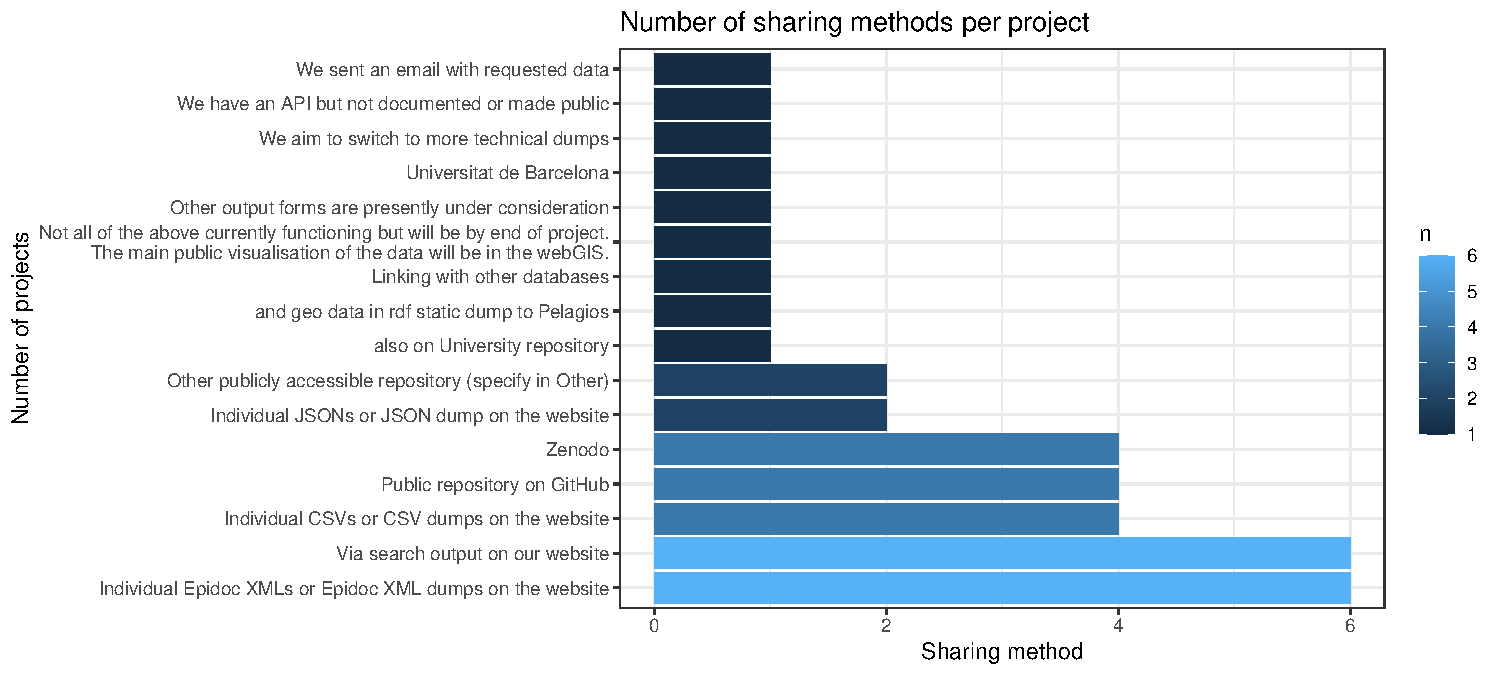
\includegraphics{01_FAIR_epi_report_files/figure-latex/fig1-1} 

}

\caption{Figure showing the popularity of individual sharing methods and formats across partner projects.}\label{fig:fig1}
\end{figure}

\normalsize

As seen in \textbf{Figure 1}, direct download of the Epidoc XML is by
far the most popular format for data sharing (implemented by 6
projects), however other Open Science services are starting to make
their way into established digital epigraphy projects, such as sharing
via a public repository, implemented by 4 (GitHub) and 4 (Zenodo)
projects respectively, as well as providing raw data in the CSV
(comma-separated value) format (4 projects), or as JSON (JavaScript
Object Notation) files (2 projects). A minority of participating partner
projects shares the data on an on-demand basis or have a non-public API
access point to their data.

\hypertarget{institutional-policies}{%
\section{Institutional policies}\label{institutional-policies}}

\textbf{Question:} \emph{Does your institution or funding body require
your project to comply with any data policies (e.g.~FAIR principles,
data storage, data sharing, Open Science)?}

\footnotesize

\begin{longtable}[]{@{}
  >{\raggedright\arraybackslash}p{(\columnwidth - 4\tabcolsep) * \real{0.9091}}
  >{\raggedleft\arraybackslash}p{(\columnwidth - 4\tabcolsep) * \real{0.0303}}
  >{\raggedleft\arraybackslash}p{(\columnwidth - 4\tabcolsep) * \real{0.0606}}@{}}
\toprule
\begin{minipage}[b]{\linewidth}\raggedright
policies
\end{minipage} & \begin{minipage}[b]{\linewidth}\raggedleft
n
\end{minipage} & \begin{minipage}[b]{\linewidth}\raggedleft
ratio
\end{minipage} \\
\midrule
\endhead
Yes & 7 & 54 \\
No & 3 & 23 \\
Not yet & 1 & 8 \\
The ERC open data policies don't apply to this project, but we are
following them anyway. & 1 & 8 \\
This is an objective, but not currently a requirement of the project. &
1 & 8 \\
\bottomrule
\end{longtable}

\normalsize

\textbf{Commentary}: The majority of projects (represented by 54\%) are
required to comply with data-related policy introduced either by their
institution or a funding body. 47\% of partner projects are not required
to follow any data policy, but some follow one on a voluntary basis.

\begin{center}\rule{0.5\linewidth}{0.5pt}\end{center}

\textbf{Question}: \emph{If you have answered YES in the previous
question, please specify what are the policies, or provide a link.}

\footnotesize

\begin{longtable}[]{@{}
  >{\raggedright\arraybackslash}p{(\columnwidth - 0\tabcolsep) * \real{1.0000}}@{}}
\toprule
\begin{minipage}[b]{\linewidth}\raggedright
policy\_specified
\end{minipage} \\
\midrule
\endhead
The funding body (the ERC) expects that research results are available
in open access \\
Open access publication. \\
Actualització de la Política d'Accés Obert a la Universitat de Barcelona
(\url{http://hdl.handle.net/2445/142065}) \\
Data Sharing, Open Science \\
usual ERC requirements \\
Currently subject to ERC open data policies
(\url{https://ec.europa.eu/research/participants/docs/h2020-funding-guide/cross-cutting-issues/open-access-data-management/open-access_en.htm});
previously Oxford University open data policies (which mirror UKRI
policies:
\url{https://www.ukri.org/publications/ukri-open-access-policy/}) \\
\url{https://forschungsdatenmanagement.bbaw.de/de} \\
\bottomrule
\end{longtable}

\normalsize

\textbf{Commentary}: Several of the partner projects follow the ERC data
and open access policies. More information on ERC Open Research Data and
Data Management Plans can be found at
\url{https://erc.europa.eu/sites/default/files/document/file/ERC_info_document-Open_Research_Data_and_Data_Management_Plans.pdf}
or at ERC Open Science policies page
\url{https://erc.europa.eu/managing-your-project/open-science}.

\hypertarget{open-science-practice}{%
\section{Open Science practice}\label{open-science-practice}}

\textbf{Question}: \emph{Standardized terminologies: The project uses
the following systems:}

\footnotesize

\begin{longtable}[]{@{}
  >{\raggedright\arraybackslash}p{(\columnwidth - 4\tabcolsep) * \real{0.9627}}
  >{\raggedleft\arraybackslash}p{(\columnwidth - 4\tabcolsep) * \real{0.0124}}
  >{\raggedleft\arraybackslash}p{(\columnwidth - 4\tabcolsep) * \real{0.0249}}@{}}
\toprule
\begin{minipage}[b]{\linewidth}\raggedright
standard\_terminologies
\end{minipage} & \begin{minipage}[b]{\linewidth}\raggedleft
n
\end{minipage} & \begin{minipage}[b]{\linewidth}\raggedleft
ratio
\end{minipage} \\
\midrule
\endhead
Internal authority lists & 8 & 62 \\
Own version of EAGLE vocabularies (edited for our project) & 7 & 54 \\
EAGLE vocabularies as provided at
\url{https://www.eagle-network.eu/resources/vocabularies/} & 5 & 38 \\
Other: ``Pre-defined lists are a problem in itself as it is difficult to
categorize in advance everything what may be found in real life. Besides
there often are open questions. Flexibility and openness for real
evidence is needed.'' & 1 & 8 \\
Other: \url{http://kerameikos.org/} for vase forms & 1 & 8 \\
Other: Language of publication is Latin & 1 & 8 \\
Other: use of
\url{https://www.getty.edu/research/tools/vocabularies/aat/} where EAGLE
is deficient & 1 & 8 \\
\bottomrule
\end{longtable}

\normalsize

\textbf{Commentary}: Internal authority lists are the most widely used
method to record epigraphic terminologies (62 \% of projects). The
vocabularies for the epigraphic discipline created by the EAGLE project
(\url{https://www.eagle-network.eu/resources/vocabularies/}) are used
either in their original form (38\% of participating projects) or in a
form modified for the individual needs of the project (54\% of
participating projects). The use of non-standardized internal authority
lists and the need for modifications suggests that the EAGLE
vocabularies do not in fact offer sufficiently a community-wide standard
and need to be improved before becoming one. This process has been
already started by the Epigraphy.info Vocabularies working group of
which Hermankova, Horster, and Prag are all members. For more details
see \url{https://epigraphy.info/vocabularies_wg/}. If you would like to
join the working group, please get in touch with the authors.

\begin{center}\rule{0.5\linewidth}{0.5pt}\end{center}

\textbf{Question}: \emph{Standardized terminologies: data on combination
of vocabularies systems}

\footnotesize

\begin{longtable}[]{@{}rrr@{}}
\toprule
standard\_method\_no & n & ratio \\
\midrule
\endhead
1 & 6 & 46 \\
2 & 4 & 31 \\
3 & 2 & 15 \\
4 & 1 & 8 \\
\bottomrule
\end{longtable}

\normalsize

\textbf{Commentary}: The majority of projects (46\%) use only one method
to record their standard terminologies, while 54\% of projects use a
combination of two or more methods. Internal authority lists are used in
combination with the EAGLE vocabularies both in their original and
modified form. Sharing or publication of internal authority lists would
therefore be highly beneficial for improving the existing EAGLE
vocabularies.

\begin{center}\rule{0.5\linewidth}{0.5pt}\end{center}

\textbf{Question}: \emph{Linked Open Datasets: The project uses the
following systems:}

\footnotesize

\begin{longtable}[]{@{}
  >{\raggedright\arraybackslash}p{(\columnwidth - 4\tabcolsep) * \real{0.8800}}
  >{\raggedleft\arraybackslash}p{(\columnwidth - 4\tabcolsep) * \real{0.0200}}
  >{\raggedleft\arraybackslash}p{(\columnwidth - 4\tabcolsep) * \real{0.1000}}@{}}
\toprule
\begin{minipage}[b]{\linewidth}\raggedright
linked\_data
\end{minipage} & \begin{minipage}[b]{\linewidth}\raggedleft
n
\end{minipage} & \begin{minipage}[b]{\linewidth}\raggedleft
ratio\_all\_proj
\end{minipage} \\
\midrule
\endhead
Trismegistos & 10 & 77 \\
Pleiades & 9 & 69 \\
EAGLE vocabularies & 7 & 54 \\
PIR & 4 & 31 \\
EDH People & 2 & 15 \\
LGPN & 2 & 15 \\
Other: Adriatlas & 1 & 8 \\
Other: Cartapulia & 1 & 8 \\
Other: \url{http://kerameikos.org/} & 1 & 8 \\
Other: More under consideration. Trismegistos is not free! & 1 & 8 \\
Other: OxREP mines database & 1 & 8 \\
Other: Publication is in complete sentences and descriptions which would
first have to be converted into linked open reference data & 1 & 8 \\
Other: We provide TM references in our bibliography but inconsistently
and without cross linking & 1 & 8 \\
Other: We were working on a cooperation with TM when our funding
finished & 1 & 8 \\
Period.O & 1 & 8 \\
\bottomrule
\end{longtable}

\normalsize

\textbf{Commentary}: From the listed Linked Open Datasets (LOD),
Trismegistos and Pleiades are by far the most popular, being used in
77\% and in 69\% of all participating projects. The EAGLE vocabularies
are used in 54\% of all participating projects.

\footnotesize

\normalsize

The group of LOD resources focusing on \textbf{geographic data}
(e.g.~Pleiades, Adriatlas, Cartapulia, Trismegistos) seems to be
strongly represented amongst participating projects (92 \% use at least
one of them), suggesting that geographic LOD are well established for
the study of the ancient world.

\textbf{Prosopographic data}, as represented by EDH People, PIR, and
LGPN are used by 46\% of all participating projects. The survey
responses suggest there is a great space for improvement and potentially
great benefit in creating and further improving prosopographic LOD.

\hypertarget{non-partnered-epigraphy-projects}{%
\chapter{Non-partnered epigraphy
projects}\label{non-partnered-epigraphy-projects}}

This section summarises the results of the online survey
\href{https://github.com/FAIR-epigraphy/scoping_survey_report/data/02_Survey_projects_questions.pdf}{\emph{Digital
epigraphy in 2022: scoping survey}} targeted at digital projects
currently listed under Digital Epigraphy Projects on the Digital
Classicist Wiki page
(\url{https://wiki.digitalclassicist.org/Category:Projects}) and which
was possible to trace in February 2022. The survey was sent to 83
projects and the link circulated until mid-April 2022. We have received
27 responses to the survey, a response rate of 31\%. Some participants
contributed on behalf of multiple projects in one response, which we
were unable to disentangle and thus the response rate is slightly
skewed. 96\% (26) of non-partnered projects gave consent to publish
their anonymised responses as part of the current report. The remaining
responses are excluded from the report but will be used to inform the
FAIR Epigraphy planning and decision making.

The respondents represent a wide range of projects from well established
projects to short-term PhD projects, with the average duration of a
project being 5.5 years. The shortest participating project reported
their duration as 1 year and the longest 117 years.

\textbf{Question}: \emph{Is the project still active?}

\footnotesize

\begin{longtable}[]{@{}lrr@{}}
\toprule
status & n & ratio \\
\midrule
\endhead
Yes & 19 & 73 \\
Currently not, but we are considering a re-start & 4 & 15 \\
No, the project is closed & 3 & 12 \\
\bottomrule
\end{longtable}

\normalsize

\textbf{Commentary}: 73\% of responding projects are still active, while
12\% of projects are permanently closed and do not consider restarting
in the future. 15\% of projects are currently not active, but might be
reactivated in the future.

\hypertarget{language-coverage-1}{%
\section{Language coverage}\label{language-coverage-1}}

\textbf{Question:} \emph{What is the predominant language of epigraphic
data in your project (for mixed collections or collections where other
languages are predominant provide details in Other)}

\footnotesize

\begin{longtable}[]{@{}lrr@{}}
\toprule
language & n & ratio \\
\midrule
\endhead
Greek & 16 & 38 \\
Latin & 11 & 26 \\
Phoenician & 2 & 5 \\
Akkadian & 1 & 2 \\
Ancient Languages of the Mediterranean area & 1 & 2 \\
Arabic & 1 & 2 \\
Aramaic & 1 & 2 \\
Hattian u.a. & 1 & 2 \\
Hittite & 1 & 2 \\
Hurrian & 1 & 2 \\
Luwian & 1 & 2 \\
Neopunic & 1 & 2 \\
Other & 1 & 2 \\
Palaeo-European & 1 & 2 \\
Palaeo-Hispanic & 1 & 2 \\
Punic & 1 & 2 \\
\bottomrule
\end{longtable}

\normalsize

\footnotesize

\normalsize

\textbf{Commentary:} The language coverage of the participating projects
consisted predominantly of Latin and Greek projects, representing 64\%
of projects combined. Greek is the most frequent language, either as the
sole/predominant language (11 projects) or in combination with other
languages (5 projects). Latin is the sole/predominant language in 6
projects or in combination with other languages (5 projects). 18
participating projects record inscriptions in one language only, while 8
contain inscriptions in two or more languages (5 being the maximum
number of listed languages.).

The languages listed as \texttt{Other} consisted of languages such as
Phoenician, Akkadian, Ancient Languages of the Mediterranean area,
Arabic, Aramaic, Hattian u.a., Hittite, Hurrian, Luwian, Neopunic,
Other, Palaeo-European, Palaeo-Hispanic, Punic. All languages come from
the wider Mediterranean/European linguistic space.

\textbf{Unique combinations of languages as retrieved from the survey:}

\footnotesize

\begin{longtable}[]{@{}l@{}}
\toprule
unique(projects\$Language\_clean) \\
\midrule
\endhead
Latin \\
Greek \\
Greek; Latin; Other \\
Latin; Greek \\
Hittite; Akkadian; Hurrian; Luwian; Hattian u.a. \\
Greek; Latin; Aramaic; Phoenician; Arabic \\
Greek; Latin \\
Phoenician; Punic; Neopunic \\
Palaeo-European; Palaeo-Hispanic \\
Ancient Languages of the Mediterranean area \\
\bottomrule
\end{longtable}

\normalsize

\hypertarget{it-infrastructure-1}{%
\section{IT infrastructure}\label{it-infrastructure-1}}

\textbf{Question}: \emph{Does the project have a website?}

\footnotesize

\begin{longtable}[]{@{}lr@{}}
\toprule
Website & n \\
\midrule
\endhead
Yes & 25 \\
No & 1 \\
\bottomrule
\end{longtable}

\normalsize

\textbf{Commentary}: Almost all participating projects maintain an
online presence (as of February-April 2022).

\begin{center}\rule{0.5\linewidth}{0.5pt}\end{center}

\textbf{Question}: \emph{Does your project have an IT specialist(s)?}

\footnotesize

\begin{longtable}[]{@{}
  >{\raggedright\arraybackslash}p{(\columnwidth - 4\tabcolsep) * \real{0.9455}}
  >{\raggedleft\arraybackslash}p{(\columnwidth - 4\tabcolsep) * \real{0.0182}}
  >{\raggedleft\arraybackslash}p{(\columnwidth - 4\tabcolsep) * \real{0.0364}}@{}}
\toprule
\begin{minipage}[b]{\linewidth}\raggedright
IT\_spec
\end{minipage} & \begin{minipage}[b]{\linewidth}\raggedleft
n
\end{minipage} & \begin{minipage}[b]{\linewidth}\raggedleft
ratio
\end{minipage} \\
\midrule
\endhead
N/A & 7 & 27 \\
No & 6 & 23 \\
Yes, equivalent of part-time (\textless1.0 FTE) position & 6 & 23 \\
Yes, equivalent of full-time (1.0 FTE) position & 2 & 8 \\
depending on development steps; expertise and experience transfer also
among project staff. & 1 & 4 \\
We are in cooperation with an IT specialist (equivalent of full-time
(1.0 FTE) position) of another project who takes care of a couple of
databases. & 1 & 4 \\
We do not have an IT specialist permanently assigned to the project, but
the project has institutional support, including whatever IT support is
necessary. & 1 & 4 \\
We had one & 1 & 4 \\
We have the support of two IT specialists for maintenance and small
updates, but for every major development we need to find new funding & 1
& 4 \\
\bottomrule
\end{longtable}

\normalsize

\textbf{Commentary}: Only 8\% of projects have an equivalent of 1.0 FTE
or more IT support at their disposal. 35\% of digital projects have an
IT specialist available for at least several hours per week or share
them with other digital projects within their institution. Several
projects report difficulty with finding financial resources to support
further development and long-term sustainability of the project or even
day-to-day support. 23\% of the participating projects report that they
currently do not have any access to IT support. An additional 27\% of
projects did not indicate whether they have access to IT support because
they are no longer active. In order to understand the precise
significance of this data, it would be necessary in future surveys to
clarify the current funding status of individual projects. However, the
general trend of limited access to IT support amongst non-partnered
project stands out.

\begin{center}\rule{0.5\linewidth}{0.5pt}\end{center}

\textbf{Question}: \emph{Does your project store epigraphic data in the
following formats\ldots?}

\footnotesize

\begin{longtable}[]{@{}
  >{\raggedright\arraybackslash}p{(\columnwidth - 4\tabcolsep) * \real{0.9261}}
  >{\raggedleft\arraybackslash}p{(\columnwidth - 4\tabcolsep) * \real{0.0170}}
  >{\raggedleft\arraybackslash}p{(\columnwidth - 4\tabcolsep) * \real{0.0568}}@{}}
\toprule
\begin{minipage}[b]{\linewidth}\raggedright
format
\end{minipage} & \begin{minipage}[b]{\linewidth}\raggedleft
n
\end{minipage} & \begin{minipage}[b]{\linewidth}\raggedleft
no\_format
\end{minipage} \\
\midrule
\endhead
Epidoc XML & 6 & 1 \\
SQL or similar & 4 & 1 \\
3D models only & 1 & 1 \\
CSV, SQL or similar & 1 & 2 \\
Epidoc XML, CSV & 1 & 2 \\
Epidoc XML, JSON, RDF, CSV & 1 & 4 \\
Epidoc XML, SQL or similar & 1 & 2 \\
JSON, SQL or similar, the xml version of the data is available through
the EAGLE project & 1 & 3 \\
RDF & 1 & 1 \\
SQL or similar, We are working on providing also an Epidoc XML version
of at least the annotated texts
(\url{https://epidoc.stoa.org/gl/latest/app-epi-mycenaean.html})) & 1 &
2 \\
XML adapted from Epidoc XML & 1 & 1 \\
\bottomrule
\end{longtable}

\normalsize

\footnotesize

\normalsize

\textbf{Commentary}: The majority of projects use \texttt{Epidoc\ XML}
as their main output data format (42\% of participating projects),
either in combination with other formats or as the sole data format. SQL
and similar database formats are relatively common, in 31\% of projects.
Other data formats are represented less frequently by a small number of
projects and mostly as complementary data formats to more popular
formats such as Epidoc XML or SQL: JSON (8\%), RDF (8\%), and CSV
(12\%). 4\% of projects indicated the use of a combination of analogue
data and 3D data format. 4\% of projects indicated using their own
version of Epidoc XML, adapted to their specific needs.

19\% of projects use only one type of data format, while 23\% use two or
more data format types. The data format of the projects that are no
longer active is recorded in the following \emph{Data sharing} section,
under \emph{Closed Projects}.

\hypertarget{data-sharing-1}{%
\section{Data sharing}\label{data-sharing-1}}

\hypertarget{active-projects}{%
\subsection{Active projects}\label{active-projects}}

This section summarised only the `active' projects. For
`closed/non-active' projects, see the section below.

\footnotesize

\normalsize

\textbf{Question}: \emph{Do you share your data outside of your
project?}

\footnotesize

\begin{longtable}[]{@{}
  >{\raggedright\arraybackslash}p{(\columnwidth - 4\tabcolsep) * \real{0.9217}}
  >{\raggedleft\arraybackslash}p{(\columnwidth - 4\tabcolsep) * \real{0.0261}}
  >{\raggedleft\arraybackslash}p{(\columnwidth - 4\tabcolsep) * \real{0.0522}}@{}}
\toprule
\begin{minipage}[b]{\linewidth}\raggedright
share
\end{minipage} & \begin{minipage}[b]{\linewidth}\raggedleft
n
\end{minipage} & \begin{minipage}[b]{\linewidth}\raggedleft
ratio
\end{minipage} \\
\midrule
\endhead
Yes, under a Creative Commons license & 8 & 42 \\
Not currently, but we are thinking about it & 3 & 16 \\
so far without explicit license & 1 & 5 \\
Under demand & 1 & 5 \\
we periodically share our data with the Europeana platform & 1 & 5 \\
Yes, publishing contributions with link to the Catalogue of the projects
& 1 & 5 \\
Yes, under a Creative Commons license, and also French Etalab Licence
Ouverte / Open Licence & 1 & 5 \\
Yes, under a Creative Commons license, by login through guest password &
1 & 5 \\
Yes, under a Creative Commons license, We are linked with other
databases (Clauss \& Slabby, for instance) & 1 & 5 \\
Yes, without any license & 1 & 5 \\
\bottomrule
\end{longtable}

\normalsize

\textbf{Commentary}: As of February 2022, 19 projects participated in
the survey as active projects. The majority of active projects are
willing to share their data, representing 82\% of participating
projects. 57\% of active projects share data under a Creative Commons
license, which is the preferred mode according to the FAIR data
principles. 10\% of active projects share data without any specific
license, while 5\% provide data only on demand.

\begin{center}\rule{0.5\linewidth}{0.5pt}\end{center}

\textbf{Question}: \emph{How do you share your data with users outside
your project?}

\footnotesize

\begin{longtable}[]{@{}
  >{\raggedright\arraybackslash}p{(\columnwidth - 4\tabcolsep) * \real{0.9490}}
  >{\raggedleft\arraybackslash}p{(\columnwidth - 4\tabcolsep) * \real{0.0096}}
  >{\raggedleft\arraybackslash}p{(\columnwidth - 4\tabcolsep) * \real{0.0414}}@{}}
\toprule
\begin{minipage}[b]{\linewidth}\raggedright
share\_all
\end{minipage} & \begin{minipage}[b]{\linewidth}\raggedleft
n
\end{minipage} & \begin{minipage}[b]{\linewidth}\raggedleft
share\_method
\end{minipage} \\
\midrule
\endhead
Individual Epidoc XMLs or Epidoc XML dumps on the website & 2 & 1 \\
Via search output on our website & 2 & 1 \\
depending of the request & 1 & 1 \\
Individual CSVs or CSV dumps on the website & 1 & 1 \\
Individual Epidoc XMLs or Epidoc XML dumps on the forthcoming website
and GitHub & 1 & 1 \\
Individual Epidoc XMLs or Epidoc XML dumps on the website, We sent an
email with requested data & 1 & 2 \\
on request & 1 & 1 \\
Other publicly accessible repository (specify in Other),
\url{http://repository.edition-topoi.org/collection/ICG} & 1 & 2 \\
Other publicly accessible repository (specify in Other), Individual
JSONs or JSON dump on the website, Individual Epidoc XMLs or Epidoc XML
dumps on the website, Public API on our website, French Huma-Num
platform and services, particularly Nakala services for our photographs
(\url{https://nakala.fr/}) & 1 & 6 \\
Other publicly accessible repository (specify in Other), We have a
DSpace instance for sharing project data. At present we are behind on
putting material on the externally accessible database because of
complications in moving to an EpiDoc-based metadata system. & 1 & 2 \\
Public repository on GitHub, Individual Epidoc XMLs or Epidoc XML dumps
on the website & 1 & 2 \\
Sketchfab website & 1 & 1 \\
Via search output on our website, We sent an email with requested data,
Research Data Repository (RDR) of the Cluster of Excellence
``Understanding Written Artefacts''; Individual Epidoc XMLs or Epidoc
XML dumps on the website is planned for the future. & 1 & 4 \\
We don't currently share data outside our project & 1 & 1 \\
We sent an email with requested data, We ar planning to have an API;
Search results can be downloaded as CSV files. & 1 & 3 \\
Zenodo, Other publicly accessible repository (specify in Other),
Individual Epidoc XMLs or Epidoc XML dumps on the website & 1 & 3 \\
Zenodo, the xml version of the data is available through the EAGLE
project & 1 & 2 \\
\bottomrule
\end{longtable}

\normalsize

\textbf{Commentary}: As of February 2022, all but one of the active
projects provide at least one way of sharing data (whether it is
currently accessible to the public or not, or it is intended to be
accessible in the future). The average (median) number of sharing
methods per project is 2, while the maximum number is 6.

There is no discipline-wide standard data repository as is common in
other disciplines (e.g.~TDAR, \url{https://core.tdar.org/}, or
AriadnePlus, \url{https://ariadne-infrastructure.eu/} for archaeological
data). Thus all projects use either their institutional or national
resources that may or may not be ideal for epigraphic data. Among those
who share data, the Epidoc XML format is the most popular format for
data sharing (14 projects), alongside providing data output upon search
on the project's website (in whichever format). Open Science practices
do not seem to be a popular choice in digital epigraphy, such as sharing
via public repository, e.g.~GitHub (2 projects) or Zenodo (2 projects),
as well as providing raw data in the CSV (comma-separated value) format,
or as JSON (JavaScript Object Notation) files. Computer-automated access
to data is rare and manual human interaction, such as manual selection
and/or manual download of files prevails, potentially hindering any
quantitative and reproducible studies, or the linking of datasets via
automated processes. For example, an API access point is currently
available only for a very limited number of projects.

\begin{center}\rule{0.5\linewidth}{0.5pt}\end{center}

\hypertarget{closed-projects}{%
\subsection{Closed projects}\label{closed-projects}}

This section summarised only the `closed/non-active' projects. For
`active' projects, see the section above.

\textbf{Question}: \emph{Is the data created by your project
accessible?}

\footnotesize

\normalsize

\footnotesize

\begin{longtable}[]{@{}
  >{\raggedright\arraybackslash}p{(\columnwidth - 4\tabcolsep) * \real{0.8714}}
  >{\raggedleft\arraybackslash}p{(\columnwidth - 4\tabcolsep) * \real{0.0429}}
  >{\raggedleft\arraybackslash}p{(\columnwidth - 4\tabcolsep) * \real{0.0857}}@{}}
\toprule
\begin{minipage}[b]{\linewidth}\raggedright
share
\end{minipage} & \begin{minipage}[b]{\linewidth}\raggedleft
n
\end{minipage} & \begin{minipage}[b]{\linewidth}\raggedleft
ratio
\end{minipage} \\
\midrule
\endhead
Yes, under a Creative Commons license & 5 & 71 \\
Not currently, but we are thinking about making it available & 1 & 14 \\
Yes, without any license & 1 & 14 \\
\bottomrule
\end{longtable}

\normalsize

\textbf{Commentary}: As of February 2022, 7 of the participating
projects are closed. 71\% of them provide access to their data under a
Creative Commons license even though the project is no longer active,
14\% of closed projects provide access without any license and 14\% do
not currently provide access to the data they have created during the
live phase of their project, but they are considering making the data
available.

\begin{center}\rule{0.5\linewidth}{0.5pt}\end{center}

\textbf{Question}: \emph{Is the data created by your project
accessible?}

\footnotesize

\begin{longtable}[]{@{}
  >{\raggedright\arraybackslash}p{(\columnwidth - 4\tabcolsep) * \real{0.9250}}
  >{\raggedleft\arraybackslash}p{(\columnwidth - 4\tabcolsep) * \real{0.0250}}
  >{\raggedleft\arraybackslash}p{(\columnwidth - 4\tabcolsep) * \real{0.0500}}@{}}
\toprule
\begin{minipage}[b]{\linewidth}\raggedright
service
\end{minipage} & \begin{minipage}[b]{\linewidth}\raggedleft
n
\end{minipage} & \begin{minipage}[b]{\linewidth}\raggedleft
ratio
\end{minipage} \\
\midrule
\endhead
Individual Epidoc XMLs or Epidoc XML dumps on the website & 4 & 57 \\
Public repository on GitHub & 3 & 43 \\
Other publicly accessible repository (specify in Other) & 2 & 29 \\
Other: \url{https://open.library.ubc.ca/collections/squeezes} & 1 &
14 \\
Other: ILC4CLARIN Repository
\url{https://dspace-clarin-it.ilc.cnr.it/repository/xmlui/handle/20.500.11752/OPEN-548}
& 1 & 14 \\
Via search output on our website & 1 & 14 \\
We don't currently share data outside our project & 1 & 14 \\
\bottomrule
\end{longtable}

\normalsize

\textbf{Commentary}: As of February 2022, 7 of the participating
projects are closed. Out of these closed projects, 57\% provide their
data in the Epidoc XML format on their website, 43\% provide their data
via public repository on GitHub, 29\% via other publicly accessible
repositories. 14\% of closed projects dot currently share data outside
the project (=1 project).

The fact that even the closed projects share their data in some form
even after the project is no longer active/does not have funding for
further development or maintenance is positive. However, most of the
data sit on private or institutional websites that can easily disappear,
along with access to the data. The best practice for the longevity of
these created datasets would be archiving them to a publicly accessible
repository, such as GitHub, Zenodo, HAL, Open Science Framework or any
similar archival infrastructure.

\begin{center}\rule{0.5\linewidth}{0.5pt}\end{center}

\hypertarget{institutional-policies-1}{%
\section{Institutional policies}\label{institutional-policies-1}}

\emph{Question:} \emph{Does your institution or funding body require
your project to comply with any data policies (e.g.~FAIR principles,
data storage, data sharing, Open Science)?}

\footnotesize

\begin{longtable}[]{@{}
  >{\raggedright\arraybackslash}p{(\columnwidth - 4\tabcolsep) * \real{0.9471}}
  >{\raggedleft\arraybackslash}p{(\columnwidth - 4\tabcolsep) * \real{0.0176}}
  >{\raggedleft\arraybackslash}p{(\columnwidth - 4\tabcolsep) * \real{0.0353}}@{}}
\toprule
\begin{minipage}[b]{\linewidth}\raggedright
policies
\end{minipage} & \begin{minipage}[b]{\linewidth}\raggedleft
n
\end{minipage} & \begin{minipage}[b]{\linewidth}\raggedleft
ratio
\end{minipage} \\
\midrule
\endhead
No & 11 & 58 \\
Yes & 3 & 16 \\
Neither our grant funding (NEH), private funding, nor institutional
funding REQUIRES compliance with data policies, but all three encourage
open data practices. & 1 & 5 \\
Not with an official request, at the moment & 1 & 5 \\
Policies are on the way, but not yet established. & 1 & 5 \\
The French National Centre for Scientific Research strongly encourages
its members to comply with the FAIR principles. & 1 & 5 \\
We don't work for any institution & 1 & 5 \\
\bottomrule
\end{longtable}

\normalsize

\textbf{Commentary}: 58\% of projects do not explicitly have to follow
any policy. 16\% of projects are required to comply with data related
policies, while an additional 20\% of projects are encouraged to comply
with FAIR data principles but no rules are enforced.

However, some of the projects are already closed and may have been
closed for some time. Data policy requirements have undergone major
changes in the last 5 years, and it is more than likely that such
policies were not previously required, which may be reflected in the
relatively low compliance with FAIR and Open Science data policies.

\begin{center}\rule{0.5\linewidth}{0.5pt}\end{center}

\textbf{Question}: \emph{If you have answered YES in the previous
question, please specify what are the policies, or provide a link.}

\footnotesize

\begin{longtable}[]{@{}
  >{\raggedright\arraybackslash}p{(\columnwidth - 2\tabcolsep) * \real{0.0118}}
  >{\raggedright\arraybackslash}p{(\columnwidth - 2\tabcolsep) * \real{0.9882}}@{}}
\toprule
\begin{minipage}[b]{\linewidth}\raggedright
\end{minipage} & \begin{minipage}[b]{\linewidth}\raggedright
policy\_example
\end{minipage} \\
\midrule
\endhead
3 &
\url{https://www.uio.no/english/for-employees/support/research/research-data-management/fair-data/} \\
6 & All : French ``Plan national pour la science ouverte:Open Science'',
\url{https://www.ouvrirlascience.fr/plan-national-pour-la-science-ouverte/};
FAIR principles, Mandatory deposit of our publications on the open
archive HAL, \url{https://hal.archives-ouvertes.fr/} \\
9 & Creative Commons \\
\bottomrule
\end{longtable}

\normalsize

\textbf{Commentary}: Data policies in the field of digital epigraphy are
still being implemented and so are not yet reflected in past and current
projects. There is a variation between national policies amongst our
responses, with France and Norway providing examples in the
implementation of Open Science in digital epigraphy.

\footnotesize

\normalsize

\footnotesize

\begin{longtable}[]{@{}lr@{}}
\toprule
policy\_simple & average\_duration\_years \\
\midrule
\endhead
N/A & 4.285714 \\
No & 10.071429 \\
Voluntary & 4.000000 \\
Yes & 35.750000 \\
\bottomrule
\end{longtable}

\normalsize

\textbf{Additional investigation}:

The main factor influencing the need to comply with institutional
principles seems to be the age of the project - for projects created in
recent years (e.g.~since 2015), we would expect FAIR data policies to be
one of conditions for securing funding. In order to verify this
hypothesis, we collected additional information manually from project
websites and published materials, such as the official project
start-date, the country of origin of a given project, indications of
existing funding and primary focus of a given project (text publication
or metadata collection). The anonymised data is saved as a TSV in the
same GitHub repository as
\texttt{/data/02\_scoping\_survey\_anonymised\_PostSurvey.tsv}.

\footnotesize

\normalsize

\footnotesize

\begin{figure}

{\centering 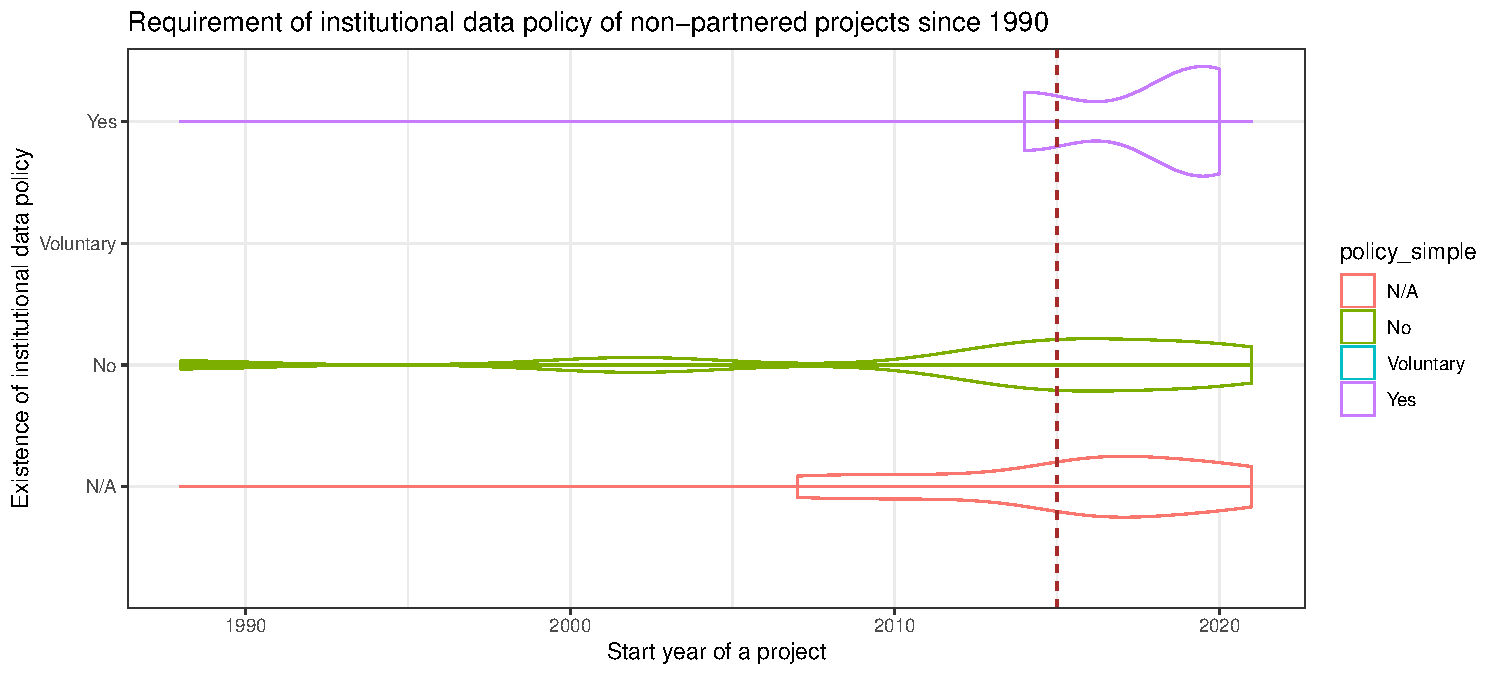
\includegraphics{01_FAIR_epi_report_files/figure-latex/fig2-1} 

}

\caption{The chart shows the existence of institutional data policy of non-partnered projects and its development over time.}\label{fig:fig2}
\end{figure}

\normalsize

Our expectations on data policies being progressively implemented over
the last seven years were confirmed only partially. As \textbf{Figure 1}
above demonstrates, the number of projects that indicated an existing
institutional data policy grows steadily from 2015 (indicated by brown
dashed vertical line). On the contrary, the number of projects that
indicated no existing data policy decreases, but only relatively slowly.
The projects responded \texttt{N/A} are those which consider themselves
in February 2022 as \texttt{closed}.

\footnotesize

\normalsize

\footnotesize

\begin{figure}

{\centering 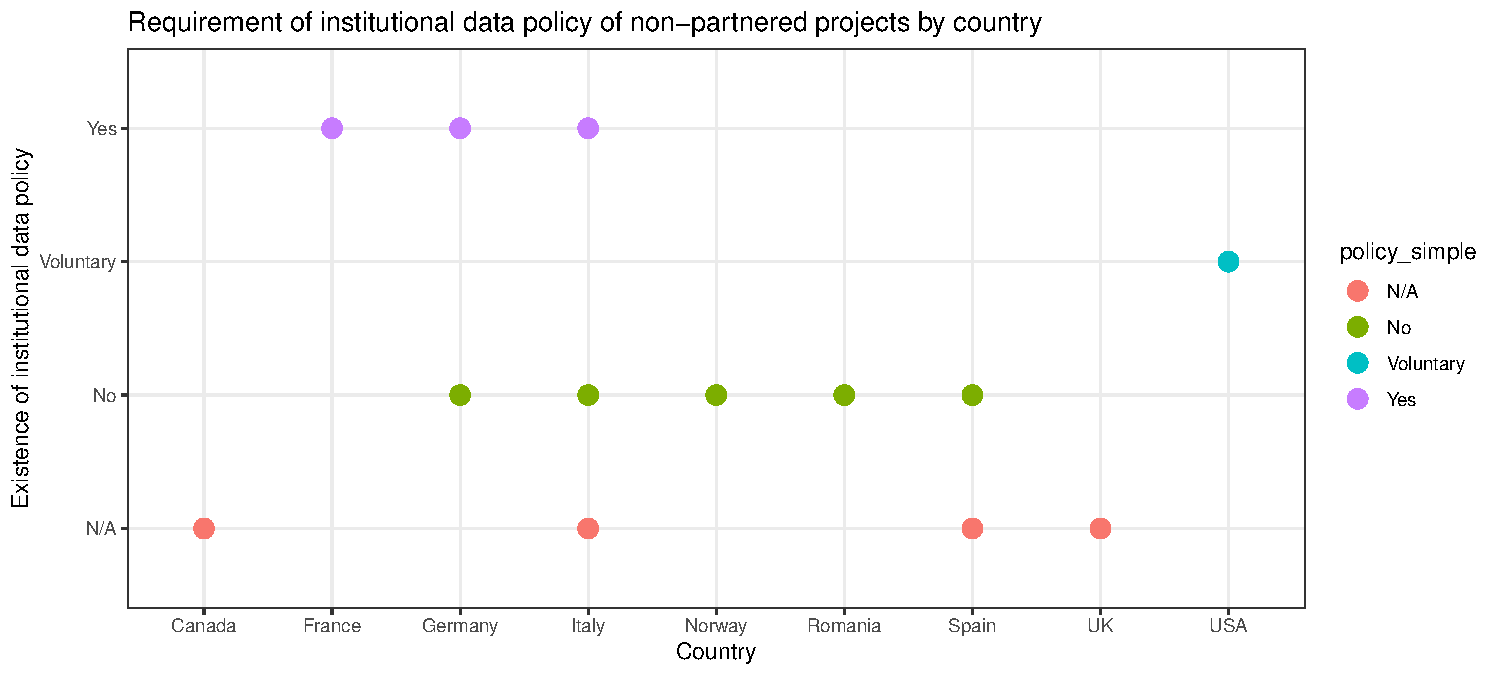
\includegraphics{01_FAIR_epi_report_files/figure-latex/unnamed-chunk-37-1} 

}

\caption{The chart shows the requirement of institutional data policy of non-partnered projects by country.}\label{fig:unnamed-chunk-37}
\end{figure}

\normalsize

\newpage

\textbf{Figure 2} above shows clear geographic differences in
implementation of data policies based on the main country where the
project is based. France, Germany, and Italy are listed as countries
where data policies are required, yet some projects in Germany and Italy
answered that no data policies are required. Thus the practical
implementation of data policies may depend on the particular funding
agency or institution, rather than on nation-wide policies. We are well
aware that data policies might be different for projects funded from
other sources than national or European research council schemes, where
such requirements may not be compulsory. Our results are only
preliminary and based on a very small sample and need to be confirmed by
further and more detailed investigation.

\hypertarget{open-science-practice-1}{%
\section{Open Science Practice}\label{open-science-practice-1}}

\textbf{Question}: \emph{Are you familiar with the FAIR data
principles?}

\footnotesize

\begin{longtable}[]{@{}lrr@{}}
\toprule
policy & n & ratio \\
\midrule
\endhead
Yes & 19 & 73 \\
Vaguely & 6 & 23 \\
No & 1 & 4 \\
\bottomrule
\end{longtable}

\normalsize

\textbf{Commentary}: The majority of projects (73\%) is familiar with
FAIR data policy, however, 23\% of participating projects are only
vaguely familiar and would benefit from clear guidelines customised for
the epigraphic community. Only 4\% of projects are not familiar with
FAIR data principles.

\begin{center}\rule{0.5\linewidth}{0.5pt}\end{center}

\textbf{Question}: \emph{Standardized terminologies: The project uses
the following systems:}

\footnotesize

\begin{longtable}[]{@{}
  >{\raggedright\arraybackslash}p{(\columnwidth - 4\tabcolsep) * \real{0.9514}}
  >{\raggedleft\arraybackslash}p{(\columnwidth - 4\tabcolsep) * \real{0.0162}}
  >{\raggedleft\arraybackslash}p{(\columnwidth - 4\tabcolsep) * \real{0.0324}}@{}}
\toprule
\begin{minipage}[b]{\linewidth}\raggedright
standard\_terminologies
\end{minipage} & \begin{minipage}[b]{\linewidth}\raggedleft
n
\end{minipage} & \begin{minipage}[b]{\linewidth}\raggedleft
ratio
\end{minipage} \\
\midrule
\endhead
Internal authority lists & 13 & 37 \\
EAGLE vocabularies as provided at
\url{https://www.eagle-network.eu/resources/vocabularies/} & 7 & 20 \\
Own version of EAGLE vocabularies (edited for our project) & 6 & 17 \\
We don't use any standardized lists & 3 & 9 \\
Other: \url{https://epigraphie.mom.fr} & 1 & 3 \\
Other: The project suggests the use of vocabularies in digital projects
dealing with ancient writing cultures {[}FAIR Epi: Not Applicable{]} & 1
& 3 \\
Other: We created our own thesaurus with OpenTheso tool (EpiVoc)
\url{https://thesaurus.mom.fr/opentheso/?idt=th61} and we aligne with
existing vocabularies (work still in progress) & 1 & 3 \\
Other: We generated a system for metadata based on the UBC library's
ability to categorize objects (it was very limited for ancient objects)
& 1 & 3 \\
Other: We use standard Mycenological terms but the community does not
yet have standardized lists. & 1 & 3 \\
Other: We use the data provided by Konkordanz der Hethitischen
Keilschrifttafeln (www.hethiter.net/hetkonk) & 1 & 3 \\
\bottomrule
\end{longtable}

\normalsize

\textbf{Commentary}: 9\% of projects do not use any standardized lists
or vocabularies. Those projects are most likely those who focus on 3D
visualisation of inscriptions or publication of metadata, rather than
publication of text editions. 37\% of projects use their own internal
authority lists. EAGLE vocabularies in their original form are used by
20\% of projects, and in an edited version by 17\% of projects. Several
projects that focus on languages other than Greek and Latin have created
their own systems, sometimes working from existing vocabularies, but
also building thesauri, e.g.~the creation of a thesaurus such as the
OpenTheso tool (EpiVoc)
\url{https://thesaurus.mom.fr/opentheso/?idt=th61} aligned with existing
vocabularies or using terms of the community.

\begin{center}\rule{0.5\linewidth}{0.5pt}\end{center}

\textbf{Question}: \emph{Are you willing to share the standardized
terminologies used in your project with us (e.g.~type of inscription
vocabularies, type of material etc.)}

\footnotesize

\begin{longtable}[]{@{}lrr@{}}
\toprule
policy\_share & n & ratio \\
\midrule
\endhead
Yes & 23 & 88 \\
No & 3 & 12 \\
\bottomrule
\end{longtable}

\normalsize

\textbf{Commentary}: The vast majority of participating projects (88\%)
is willing to share any standardized terminologies used in their
project, such as terminologies covering the type of inscription, the
type of material etc.

\begin{center}\rule{0.5\linewidth}{0.5pt}\end{center}

\textbf{Question}: \emph{Linked Open Datasets: The project uses the
following systems:}

\footnotesize

\begin{longtable}[]{@{}
  >{\raggedright\arraybackslash}p{(\columnwidth - 4\tabcolsep) * \real{0.8831}}
  >{\raggedleft\arraybackslash}p{(\columnwidth - 4\tabcolsep) * \real{0.0390}}
  >{\raggedleft\arraybackslash}p{(\columnwidth - 4\tabcolsep) * \real{0.0779}}@{}}
\toprule
\begin{minipage}[b]{\linewidth}\raggedright
linked\_data
\end{minipage} & \begin{minipage}[b]{\linewidth}\raggedleft
n
\end{minipage} & \begin{minipage}[b]{\linewidth}\raggedleft
ratio
\end{minipage} \\
\midrule
\endhead
Pleiades & 13 & 50 \\
Trismegistos & 13 & 50 \\
EAGLE vocabularies & 9 & 35 \\
LGPN & 7 & 27 \\
Other: None & 3 & 12 \\
PIR & 3 & 12 \\
Other: diacritical marks from Leiden (CIL) & 1 & 4 \\
Other: Geonames & 1 & 4 \\
Other: GODOT: \url{https://godot.date/home} & 1 & 4 \\
Other: I can't remember (sorry!) & 1 & 4 \\
Other: iDaiGazetteer & 1 & 4 \\
Other: idRef & 1 & 4 \\
Other: None were yet available - a new edition will want to use all & 1
& 4 \\
Other: Pactols & 1 & 4 \\
Other: PLRE & 1 & 4 \\
Other: ToposTexts & 1 & 4 \\
Other: under demand & 1 & 4 \\
Other: We periodically ask to Trismegistos an ID for our records & 1 &
4 \\
Period.O & 1 & 4 \\
\bottomrule
\end{longtable}

\normalsize

\textbf{Commentary}: Pleiades is the most popular LOD dataset, being
used in 50\% of all participating projects, alongside Trismegistos also
in 50\%. EAGLE vocabularies are represented in 35\% of participating
projects, while combined prosopographic datasets (LGPN+PIR) feature in
39\% of projects. Only 12\% of participating projects do not use any
LOD.

\footnotesize

\normalsize

The group of LOD resources focusing on \textbf{geographic data}
(e.g.~Pleiades, iDai Gazetteer, Geonames, Trismegistos) seems to be
strongly represented amongst participating non-partnered projects (77 \%
use at least one of them), suggesting that geographic LOD are well
established for the study of the ancient world.

\textbf{Prosopographic data}, represented by LGPN, PIR, and PLRE are
used by 35\% of all participating non-partnered projects.

\textbf{Chronological data}, represented by Period.O and GODOT are used
by 8 \% of all participating non-partnered projects.

It is worth noting that not every category listed amongst the responses
is a true linked open dataset. The survey responses suggest there is a
considerable room for improvement and potentially great benefit in
creating and further improving LOD for the study of the ancient world.

\hypertarget{future-needs-of-digital-epigraphy}{%
\chapter{Future needs of digital
epigraphy}\label{future-needs-of-digital-epigraphy}}

This section covers the wishes of all participating digital epigraphy
projects. The responses were anonymised so no individual or project can
be identified but are otherwise presented as submitted in the survey.

\hypertarget{partner-projects}{%
\section{Partner projects}\label{partner-projects}}

\textbf{Question}: \emph{Our project would like to be able to use within
the next three years:}

\footnotesize

\begin{longtable}[]{@{}
  >{\raggedright\arraybackslash}p{(\columnwidth - 4\tabcolsep) * \real{0.9627}}
  >{\raggedleft\arraybackslash}p{(\columnwidth - 4\tabcolsep) * \real{0.0124}}
  >{\raggedleft\arraybackslash}p{(\columnwidth - 4\tabcolsep) * \real{0.0249}}@{}}
\toprule
\begin{minipage}[b]{\linewidth}\raggedright
lod\_f
\end{minipage} & \begin{minipage}[b]{\linewidth}\raggedleft
n
\end{minipage} & \begin{minipage}[b]{\linewidth}\raggedleft
ratio
\end{minipage} \\
\midrule
\endhead
Bibliographical references to all epigraphic publications with stable
URI (e.g.~Zenon) & 11 & 85 \\
EAGLE vocabularies (revised and extended with clear structure +
eliminated duplicates + multi-language support) & 10 & 77 \\
Roman Prosopographical data with stable URIs & 10 & 77 \\
Greek Onomastic data with stable URIs (e.g.~LGPN with stable
identifiers) & 7 & 54 \\
Open and accessible RDF Triplestore & 7 & 54 \\
One domain specific repository for epigraphic data & 5 & 38 \\
Other: standardised terminologies for instrumentum domesticum and
palaeography & 1 & 8 \\
Other: We are not sure what is meant by ``epigraphic data'' in the
preceding entry. If something like a papyri.info for inscriptions then
no. If a basic aggregator like Humanities Commons for epigraphy then
that would be more useful. & 1 & 8 \\
\bottomrule
\end{longtable}

\normalsize

\textbf{Commentary}: The most popular is the option
\texttt{Bibliographical\ references\ to\ all\ epigraphic\ publications\ with\ stable\ URI\ (e.g.\ Zenon)},
representing the wishes of 85\% of all partner projects.

The great interest in prosopographic LOD for epigraphy is supported by
77\% of partner projects for the Roman world and 54\% of projects for
the Greek world respectively.

The \texttt{improved\ EAGLE\ vocabularies} are wished for by 77\% of
partner projects.

The \texttt{domain-specific\ repository\ for\ epigraphic\ data}
(discussed also under \texttt{Other} responses) or the
\texttt{open\ and\ accessible\ RDF\ Triplestore} do not seem to be the
highest priority of participating projects, but are still relatively
popular as 38\% of respondants wishes for one of the two. One
participating project wishes specifically for the following: Other:
standardised terminologies for instrumentum domesticum and palaeography.

\begin{center}\rule{0.5\linewidth}{0.5pt}\end{center}

\textbf{Question}: \emph{Potential ideas that our project would benefit
from:}

\footnotesize

\begin{longtable}[]{@{}
  >{\raggedright\arraybackslash}p{(\columnwidth - 4\tabcolsep) * \real{0.8022}}
  >{\raggedleft\arraybackslash}p{(\columnwidth - 4\tabcolsep) * \real{0.0330}}
  >{\raggedleft\arraybackslash}p{(\columnwidth - 4\tabcolsep) * \real{0.1648}}@{}}
\toprule
\begin{minipage}[b]{\linewidth}\raggedright
lod\_i
\end{minipage} & \begin{minipage}[b]{\linewidth}\raggedleft
n
\end{minipage} & \begin{minipage}[b]{\linewidth}\raggedleft
ratio\_all\_proj
\end{minipage} \\
\midrule
\endhead
Set of guidelines for FAIR and Linked Open Data in epigraphy & 12 &
92 \\
Practical scripted examples on how to use LOD in epigraphy & 10 & 77 \\
Workshop on FAIR principles in epigraphy & 8 & 62 \\
Workshop on how to use LOD in epigraphy & 7 & 54 \\
Set of guidelines/resources for quantitative analysis of epigraphic data
& 6 & 46 \\
NA & 1 & 8 \\
\bottomrule
\end{longtable}

\normalsize

\textbf{Commentary}: 92\% of all projects consider that they would
benefit from
\texttt{A\ set\ of\ guidelines\ for\ FAIR\ and\ Linked\ Open\ Data\ in\ epigraphy}.
There is a general interest in practical examples and workshop(s) on how
to use LOD and FAIR Principles in epigraphy, as well as resources for
quantitative analysis of data in epigraphy.

\begin{center}\rule{0.5\linewidth}{0.5pt}\end{center}

\textbf{Question}: \emph{Additional digital needs}

\footnotesize

\begin{verbatim}
## [1] "Further development of a single research portal to interrogate multiple
epigraphic databases; development of a specific API to use the standardized common
vocabularies"
## [2] "- Further collaboration and development of concepts for vocabularies. - Getty
vocabularies crosswalks where they apply - In doing all this work, we hope that FAIR
Epigraphy will use as many different applications of the EpiDoc schema as possible, so as
to accommodate the ways different projects mark up documents and metadata."
## [3] "Sustainable common platform of all digital epigraphic editions (a Vision)"
## [4] "Advisory Board for new Digital Epigraphy projects, guidelines for FAIR epigraphy"
## [5] "Standards for palaeography, prosopography, bibliograpy, instrumentum domesticum
and linguistic analysis"
## [6] "1) Provide us support in switching to Epidoc XML encoding 2) Help us clarify how
our data are accessible to the public (CC-BY 4.0) 3) Promote the sustainability of
projects whose funds have ended 4) Foster interoperability between digital resources 5)
Improve the standardization of projects in digital epigraphy"
\end{verbatim}

\normalsize

\textbf{Commentary}: This section covers the additional needs of partner
projects. Partner projects would like to see a platform linking
epigraphic data from multiple sources, including a stable reference
point or an API for improved epigraphic vocabularies (in other words,
the sort of resource which agreed vocabularies and an RDF triplestore
might facilitate). Partner projects would also like to be able to use
guidelines for FAIR practices in epigraphy, which currently do not
exist.

\hypertarget{non-partnered-projects}{%
\section{Non-partnered projects}\label{non-partnered-projects}}

\textbf{Question}: \emph{Our project would like to be able to use within
the next three years:}

\footnotesize

\begin{longtable}[]{@{}
  >{\raggedright\arraybackslash}p{(\columnwidth - 4\tabcolsep) * \real{0.8615}}
  >{\raggedleft\arraybackslash}p{(\columnwidth - 4\tabcolsep) * \real{0.0231}}
  >{\raggedleft\arraybackslash}p{(\columnwidth - 4\tabcolsep) * \real{0.1154}}@{}}
\toprule
\begin{minipage}[b]{\linewidth}\raggedright
lod\_f
\end{minipage} & \begin{minipage}[b]{\linewidth}\raggedleft
n
\end{minipage} & \begin{minipage}[b]{\linewidth}\raggedleft
ratio\_all\_proj
\end{minipage} \\
\midrule
\endhead
Bibliographical references to all epigraphic publications with stable
URI (e.g.~Zenon) & 17 & 65 \\
EAGLE vocabularies (revised and extended with clear structure +
eliminated duplicates + multi-language support) & 17 & 65 \\
Greek Onomastic data with stable URIs (e.g.~LGPN with stable
identifiers) & 13 & 50 \\
One domain specific repository for epigraphic data & 11 & 42 \\
Roman Prosopographical data with stable URIs & 11 & 42 \\
Open and accessible RDF Triplestore & 6 & 23 \\
Other: None & 2 & 8 \\
Other: Geolocation of inscriptions and searches related to geography & 1
& 4 \\
Other: In the case of our project most of the options are not applicable
& 1 & 4 \\
Other: LGPN does not yet contain Mycenaean names but I would be happy if
that changed & 1 & 4 \\
Other: This project is currently closed & 1 & 4 \\
\bottomrule
\end{longtable}

\normalsize

\textbf{Commentary}: The most popular is the option
\texttt{Bibliographical\ references\ to\ all\ epigraphic\ publications\ with\ stable\ URI\ (e.g.\ Zenon)}
representing the wishes of 65\% of all participating projects. The great
interest in onomastic and prosopographic LOD for both the Greek and
Roman world is supported by 92\% of non-partnered projects. The
\texttt{improved\ EAGLE\ vocabularies} are wished for by 65\% of
non-partnered projects. The
\texttt{domain-specific\ repository\ for\ epigraphic\ data} (23\%) or
the \texttt{open\ and\ accessible\ RDF\ Triplestore} (42\%) do not seem
to be the highest priority of participating projects, but still a
relatively popular response. One participating project wishes
specifically for the following: Other: Geolocation of inscriptions and
searches related to geography, which other existing projects, such as
Pleiades or Trismegistos, might be better equipped to provide. The
differences between the wishes and answers of the non-partnered projects
is \emph{inter alia} related to the fact that several partner projects
come from a world beyond Greek and Latin epigraphy.

\begin{center}\rule{0.5\linewidth}{0.5pt}\end{center}

\textbf{Question}: \emph{Potential ideas that our project would benefit
from:}

\footnotesize

\begin{longtable}[]{@{}
  >{\raggedright\arraybackslash}p{(\columnwidth - 4\tabcolsep) * \real{0.8626}}
  >{\raggedleft\arraybackslash}p{(\columnwidth - 4\tabcolsep) * \real{0.0229}}
  >{\raggedleft\arraybackslash}p{(\columnwidth - 4\tabcolsep) * \real{0.1145}}@{}}
\toprule
\begin{minipage}[b]{\linewidth}\raggedright
lod\_i
\end{minipage} & \begin{minipage}[b]{\linewidth}\raggedleft
n
\end{minipage} & \begin{minipage}[b]{\linewidth}\raggedleft
ratio\_all\_proj
\end{minipage} \\
\midrule
\endhead
Set of guidelines for FAIR and Linked Open Data in epigraphy & 22 &
85 \\
Practical scripted examples on how to use LOD in epigraphy & 17 & 65 \\
Set of guidelines/resources for quantitative analysis of epigraphic data
& 17 & 65 \\
Workshop on how to use LOD in epigraphy & 16 & 62 \\
Workshop on FAIR principles in epigraphy & 11 & 42 \\
In the next three years we planned a few Digital Epigraphy workshops in
the frame of the French School at Athens & 1 & 4 \\
None & 1 & 4 \\
\bottomrule
\end{longtable}

\normalsize

\textbf{Commentary}: 85\% of all non-partnered projects consider that
they would benefit from
\texttt{A\ set\ of\ guidelines\ for\ FAIR\ and\ Linked\ Open\ Data\ in\ epigraphy}.
There is a general interest in practical examples (65\%) and workshop(s)
on how to use LOD in epigraphy (62\%), as well as resources for
quantitative analysis of data in epigraphy (42\%).

\begin{center}\rule{0.5\linewidth}{0.5pt}\end{center}

\textbf{Question}: \emph{Additional digital needs}

\footnotesize

\begin{verbatim}
## [1] "Digitalization of Roman Inscriptions for dissemination and research"
## [2] "A workshop on integrating Mycenaean data into epigraphy?"
## [3] "Data retrieval also on spatial base: for example: from maps of the single
archaeological sites and single complexes (as plans or 3d scans of catacombs and
churches...). Links with the existing geographical and georeferenced resources.
Controlled and shared vocabulary about palaeographical features; Storage, search and
analysis of the 'aberrant forms' (not to be 'corrected') for Late Latin and
Late/Byzantine Greek words (and names)."
## [4] "The most important for me would be 1/ to have a more complete view of real FAIR
epigraphic projects and 2/a sustainable \"common place\" where to find resources + tools
and help + let's call it an improved EAGLE + and more \"international\""
## [5] "It would be very nice (but I might be a bit biased!) if FAIR Epigrahy would like
to help develop EFES (EpiDoc Front-End Services). For example by helping to make the
existing RDF data export functionality really usable even by less experienced people."
## [6] "I would love to see it revitalized and improved with FAIR and Linked Open Data
guidelines and other resources."
## [7] "Unicode for Punic"
## [8] "help to act in a shared dedicated academical environment and help in spreading
our results"
## [9] "FAIR Epigraphy's team can help us by providing advice on specifical topics"
## [10] "It would be useful to have an Open Access database of images of inscriptions
that are free from Copyright limits."
\end{verbatim}

\normalsize

\textbf{Commentary}: This section covers additional needs of
participating digital projects. Some of the wishes might be beyond the
scope of the FAIR Epigraphy project but the responses provide valuable
guidance and hint at some of the challenges the epigraphic discipline
will be facing in the near future. The responses may inspire other
projects with similar needs to join forces and potentially develop
solutions together. The FAIR Epigraphy project may offer one channel to
explore and collaborate on the meeting of these needs in future.

\hypertarget{summary}{%
\chapter{Summary}\label{summary}}

The present report demonstrates a great variation in the epigraphic
discipline in 2022. We received answers from 13 partner projects and 27
non-partnered projects. Although it may seem that a relatively small
number of projects participated in the survey, nontheless, we consider
that responses provide a representative sample of the current state of
the discipline. The response rate of non-partnered projects was lower
than the response rate of partner projects (100 \% vs 31 \%). This may
reflect the overall lower rate of compliance with FAIR principles, or
the fact that non-partnered projects may have ceased active operation
before FAIR principles were established and implemented by their
institutions and funding bodies.

The responses represent a diverse selection of projects, based mostly in
Europe and the USA. The majority of projects focus predominantly on
publication of textual editions of inscriptions (where Epidoc XML is the
main data format), while some focus on publication of related metadata
without producing new editions of text (and thus use different data
formats than Epidoc XML).

Although the majority of participating projects record inscriptions in
Latin and Greek, we see a diverse array of projects expanding beyond the
traditional focus of the discipline the way as it was established in the
19th century. The projects participating in the survey include
well-established projects that have existed over several decades,
regional or thematic corpora, and more specialised, short-term PhD
projects. We have observed a clear distinction between, on the one hand,
projects with a long tradition and most importantly with relatively
stable institutional support, which have access to institutional
repositories, policies and at least basic IT services; and on the other,
small-scale projects with limited support and access to resources and
training, typified by short-term projects on a specific topic that may
lack access to long-term institutional support. One of the missions of
the FAIR Epigraphy Project is to support projects with limited access to
resources, as well as established projects, by providing accessible and
comprehensible training and guidelines for FAIR and Linked Open Data
principles in epigraphy.

The established projects mostly follow the FAIR principles, although to
a variable extent. The majority of established projects share their data
under a Creative Commons license in one or more widely accepted formats
(with Epidoc XML being the most popular format for all types of projects
irrespective of their status and longevity). In general, the more
established projects provide more access points to their data as well as
more data formats than the projects with less institutional support. The
use of standardized terminologies is still limited and project-specific,
mostly due to the lack of uniformly accepted standards. On contrary, the
adoption of Linked Open Datasets (LOD) and creation of links within the
epigraphic datasets with stable identifiers to those LOD sources seems
to be fairly advanced, especially in the case of well-established LOD
domains such as Pleiades or Trismegistos for Graeco-Roman projects, and
to a lesser extent the EAGLE vocabularies.

The non-partnered projects follow the FAIR principles, but to a lesser
degree than the established projects. There are, however, some
short-term projects that fulfill or exceed the requirements for Open
Science, but as a general rule the compliance is lower than in the case
of established projects. The reason for lower compliance in some
projects is most likely a combination of short-term institutional
support, limited access to IT support and poor accessibility of
guidelines and discipline-specific training.

As to the current and future needs of digital epigraphy, there is a
clear demand for more and better LOD. The requests concerned especially
bibliographical references to standard epigraphic corpora,
standardisation of discipline-specific vocabularies, and prosopographic
LOD for the ancient world. In addition, there is a wish for support by
training and the provision of accessible resources and guidelines for
FAIR and Open epigraphy.

In the near future, we plan to undertake several in-depth interviews
with our partners to confirm some of our assumptions and to draft a
concrete plan for the following three years. However, it is clear from
the survey responses, that we should direct our attention to three main
tasks:

\begin{enumerate}
\def\labelenumi{\arabic{enumi}.}
\tightlist
\item
  implementing and hosting standards for epigraphic vocabularies
  (e.g.~inscription type, material, object etc.)
\item
  implementing and hosting standards for bibliographical records
  (e.g.~stable and unique records for all major epigraphic editions)
\item
  building a platform for FAIR and Open Epigraphy on the infrastructure
  provided by the University of Oxford (CSAD), that will function as an
  information hub, providing not only training and good practice
  examples, but also hosting the resources and tools.
\end{enumerate}

We hope to run a similar survey annually to track any progress within
the discipline and closely monitor changing needs of individual projects
in digital epigraphy.

\hypertarget{bibliography}{%
\chapter{Bibliography}\label{bibliography}}

\hypertarget{refs}{}
\begin{CSLReferences}{1}{0}
\leavevmode\vadjust pre{\hypertarget{ref-assael_restoring_2022}{}}%
Assael Y., Sommerschield T., Shillingford B., Bordbar M., Pavlopoulos
J., Chatzipanagiotou M., Androutsopoulos I., Prag J. \& Freitas N. de
(2022). Restoring and attributing ancient texts using deep neural
networks. Nature 603 (7900): 280--283.
\url{https://doi.org/10.1038/s41586-022-04448-z}.

\leavevmode\vadjust pre{\hypertarget{ref-bagnall_pleiades_2006}{}}%
Bagnall R., Talbert R.J.A., Bond S., Becker J., Elliott T., Gillies S.,
Horne R., McCormick M., Rabinowitz A., Turner B. \& Twele R. (2006).
Pleiades: {A} community-built gazetteer and graph of ancient places.
\url{http://pleiades.stoa.org}.

\leavevmode\vadjust pre{\hypertarget{ref-bruun_epigraphy_2015}{}}%
Elliott T. (2015). Epigraphy and {Digital} {Resources}. Vol. 1. Oxford
University Press.
\url{https://doi.org/10.1093/oxfordhb/9780195336467.013.005}.

\leavevmode\vadjust pre{\hypertarget{ref-geser_wp15_2016}{}}%
Geser G. (2016). {WP15} {Study}: {Towards} a {Web} of {Archaeological}
{Linked} {Open} {Data}. Ariadne.
\url{http://legacy.ariadne-infrastructure.eu/wp-content/uploads/2019/01/ARIADNE_archaeological_LOD_study_10-2016.pdf}.

\leavevmode\vadjust pre{\hypertarget{ref-glomb_popularity_2022}{}}%
Glomb T., Kaše V. \& Heřmánková P. (2022). Popularity of the cult of
{Asclepius} in the times of the {Antonine} {Plague}: {Temporal} modeling
of epigraphic evidence. Journal of Archaeological Science: Reports 43:
103466. \url{https://doi.org/doi.org/10.1016/j.jasrep.2022.103466}.

\leavevmode\vadjust pre{\hypertarget{ref-hermankova_inscriptions_2021}{}}%
Heřmánková P., Kaše V. \& Sobotkova A. (2021). Inscriptions as data:
Digital epigraphy in macro-historical perspective. Journal of Digital
History 1. \url{https://journalofdigitalhistory.org/en/issue/jdh001}.

\leavevmode\vadjust pre{\hypertarget{ref-mullen_manual_2021}{}}%
Mullen A. \& Bowman A.K. (2021). Manual of {Roman} everyday writing
{Volume} 1 {Volume} 1.
\url{https://latinnow.files.wordpress.com/2021/11/latinnow-mullen-and-bowman-2021-mrew-scripts-and-texts-1.pdf}.

\leavevmode\vadjust pre{\hypertarget{ref-orlandi_digital_2021}{}}%
Orlandi S. (2021). Digital {Projects} in {Epigraphy}: {Research}
{Needs}, {Technical} {Possibilities}, and {Funding} {Problems}. In:
Velasquéz Soriano I. \& Espinosa Espinosa D. (eds.). Epigraphy in the
{Digital} {Age} : {Opportunities} and challenges in the {Recording},
{Analysis} and {Dissemination} of {Inscriptions}. Archaeopress, Oxford,
p. 1--8.

\leavevmode\vadjust pre{\hypertarget{ref-roueche_inscriptions_2022}{}}%
Roueche C. (2022). Inscriptions of {Roman} {Tripolitania} 2021. The
Society for Libyan Studies.

\leavevmode\vadjust pre{\hypertarget{ref-roueche_inscriptions_2020}{}}%
Roueche C., Reynolds J. \& Bodard G. (2020). Inscriptions of {Roman}
{Cyrenaica} (2020). The Society for Libyan Studies.

\leavevmode\vadjust pre{\hypertarget{ref-tupman_where_2021}{}}%
Tupman C. (2021). Where {Can} {Our} {Inscriptions} {Take} {Us}?
{Harnessing} the {Potential} of {Linked} {Open} {Data} for {Epigraphy}.
In: Velasquéz Soriano I. \& Espinosa Espinosa D. (eds.). Epigraphy in
the {Digital} {Age} : {Opportunities} and {Challenges} in the
{Recording}, {Analysis} and {Dissemination} of {Inscriptions}.
Archaeopress, Oxford, p. 115--128.

\leavevmode\vadjust pre{\hypertarget{ref-wilkinson_fair_2016}{}}%
Wilkinson M.D., Dumontier M., Aalbersberg Ij.J., Appleton G., Axton M.,
Baak A., Blomberg N., Boiten J.-W., Silva Santos L.B. da, Bourne P.E.,
Bouwman J., Brookes A.J., Clark T., Crosas M., Dillo I., Dumon O.,
Edmunds S., Evelo C.T., Finkers R., Gonzalez-Beltran A., Gray A.J.G.,
Groth P., Goble C., Grethe J.S., Heringa J., Hoen P.A.C. 't, Hooft R.,
Kuhn T., Kok R., Kok J., Lusher S.J., Martone M.E., Mons A., Packer
A.L., Persson B., Rocca-Serra P., Roos M., Schaik R. van, Sansone S.-A.,
Schultes E., Sengstag T., Slater T., Strawn G., Swertz M.A., Thompson
M., Lei J. van der, Mulligen E. van, Velterop J., Waagmeester A.,
Wittenburg P., Wolstencroft K., Zhao J. \& Mons B. (2016). The {FAIR}
{Guiding} {Principles} for scientific data management and stewardship.
Scientific Data 3 (1): 160018.
\url{https://doi.org/10.1038/sdata.2016.18}.

\leavevmode\vadjust pre{\hypertarget{ref-willi_manual_2021}{}}%
Willi A. (2021). Manual of {Roman} everyday writing {Volume} 2 {Volume}
2.
\url{https://latinnow.files.wordpress.com/2021/06/willi-2021-writing-equipment-latinnow.pdf}.

\end{CSLReferences}

\end{document}
